%
\documentclass[11pt]{article}
\usepackage{amssymb}
\usepackage{amsmath}
\usepackage{amsthm}
\usepackage{pst-all}
\usepackage{newicktree}
\usepackage{graphicx}
\usepackage[left=1.4in,right=1.4in,top=1in,bottom=1in,includeheadfoot]{geometry}
\usepackage{setspace}
\usepackage{natbib}

\newtheorem{theorem}{Theorem}
\newtheorem{corr}{Corollary}
\newtheorem{assumptions}{Assumptions}
\newtheorem{definition}{Definition}

\DeclareMathOperator*{\argmax}{arg\,max} 

\frenchspacing
\linespread{1.25}
\parskip= 2 pt

\title{Foundations of the Age-Area Hypothesis}
\author{\textbf{Matthew J. Baker} \\ Department of Economics \\ Hunter College and the Graduate Center, CUNY}

\begin{document}

\maketitle
\begin{abstract}
\noindent Historical mass migrations have played a seminal role in shaping the global distribution of cultures. A commonly used tool in theorizing about the nature and origins of mass migrations is the so-called Age-Area Hypothesis, originally advanced by Sapir (1915). The Hypothesis posits that the origin point of a linguistic/cultural stock is most likely where the languages comprising the stock are most divergent. While compelling and often-corroborated with evidence, the Age-Area Hypothesis has never been founded in basic principles. In this paper I\ describe a micro-founded model of the Age-Area Hypothesis and present an Age-Area Theorem. I also develop an algorithm for computing the probability that any location is the point of origin for a group of related cultures. I conclude the paper with an application to the Na Dene language group. 
\end{abstract}
\newpage

The Age-Area Hypothesis - evidently first developed and applied by Sapir (1916) in his study of Native American Languages and cultures- is often invoked when linguistic
evidence is used in support of hypotheses about where different sorts of cultures originated, how they evolved over time, and how they came to be located where they are today.\footnote{One must be careful in invoking ``the'' Age-Area Hypothesis. As I will elaborate below, this paper concerns what might be called the Linguistic Age-Area Hypothesis - not the related Age-Area Hypothesis that posits the wider the distribution of a cultural trait, the older it likely is.} Briefly stated, the hypothesis says that the geographic area where a language phylogeny originated is most likely the place where the component languages of the phylogeny are most divergent, or maximally differentiated.



While the question may some of academic interest only, a wide variety of recent economic literature highlights the importance of understanding how we arrived at the current cultural mix around the globe. Coincident with this understanding is the realization that understanding where different cultures came from, and how they interacted in the past, is also of paramount importance.

Examples of the application of the linguistic age-area hypothesis  abound. Sapir himself used these arguments to suggest that the so-called Na-Dene linguistic grouping originated in and around the North West Coast. As another example, Atkinson and Gray (2003) have used the results to suggest that the Indo-European languages originated in Anatolia, not, as is sometimes supposed, on the steppes of Siberia. Further applications of the idea - either implicit or explicit use of the idea - are almost too numerous to mention. Ruhlen (2001) uses the age-area hypothesis to lend insight into debates about the origins of the Na-Dene, as well as the origins of the Bantu linguistic group in Africa.
More specifically, Darden (2001) uses the AAH extensively to buttress his picture of Ancient African History. 

What is the existing theoretical basis for the age-area hypothesis? In spite of its wide range of applications and deep implications for human history, there is, to my knowledge, no theoretical basis for the hypothesis. In population genetics, it is well-known that
the point of maximal genetic diversity of populations is closest to the geographical point of origin. For example, it is known that the domestic cat originated in Egypt because the genetic pool is deepest and most varied in Egypt. Migrant populations only carry off a subset of the genes of the parent population and hence are less diverse in a well-defined sense. 

These principles certainly do not apply to language and linguistic drift. While there are many striking parallels between the evolution of language and population genetics, they do not apply in this case. A migratory group does not carry off only a fraction of the grammar, vocabulary, or language structure of its parent! 

The lack of a theoretical basis for the  age area hypothesis is also a problem for its use in technical situations. For example, suppose one wished to include an ancient migratory path in a statistical model of migration, or that one wanted to integrate migration into a larger statistical model. Since the hypothesis has no theoretical underpinnings, it is difficult to see how to construct a likelihood for a certain path or migratory history.

In this paper, I develop a theoretical foundation for the age-area hypothesis, and make some of the terms supporting the hypothesis more rigorous. The model is micro-founded in the sense that it can be based on microeconomic principles and an associated back story. 

The theory can then be rendered in such a fashion that it turns out with a probabilistic notion of parsimony and Occam's razor; that is, when adapted in a particular fashion, migratory paths that originate at deeper points in a phylogenetic tree can be thought of as simpler in a well-structured way.  These ideas lead to a particular definition of divergence or dissimilarity for each constituent culture in the phylogeny. 

Assembling the aforementioned methods, I then develop an Age-Area Theorem, which says that a culture that is more linguistically divergent from the others in the stock is also more likely to be the point of origin of the stock. I then present a computational algorithm which relies upon backwards traversal of the tree, along with some extensions of the model. I conclude by discussing some applications.

\section{Related Literature}

\cite[p.12]{trask00} attributes the (Linguistic) Age-Area Hypothesis - also called the center-of-gravity principle, the genetic diversity principle, and Sapir's principle - to the work of Latham (1851, 1862) and Sapir (1916). He also notes that Mallory (1997) and Nichols (1997a) have qualified it in various ways.   \citet[p.336]{dimmendaal11} expresses some doubts about the exact origins of the AAH, referring to it as the ``principle of least effort'', and going on to note that ``This principle probably was applied first by the scholars working no Amerindian Languages, e.g. \cite{sapir16} and Dyen (1956)

The AAH attended to in this paper shouldn't be confused with the Sapir-Whorf Hypothesis or what could be called the Cultural Age Area Hypothesis. 



\section{Problem Description and Motivation}

I first describe the basic logic of the theorem within the confines of a simple example. Consider the hypothetical phylogenetic tree displayed in figure \ref{fig1}. The figure depicts the genetic relationship between five related cultures.  In the usual lingo, A is the `most divergent,' with B, C, D, E all being more closely related. D and E are the most closely related cultures. To avoid forming impressions based on evidence that is not part of the hypothesis, we will suppose that the locations of the
groups have been concealed from us, and that we have no access to archaeological or historical information about the language stock or any information about how the cultural stock came to be in its current locational distribution.

The Age-Area hypothesis (henceforth the AAH) posits that the point of origin of the cultural group was A's current location, as A is the most divergent language from the group.\footnote{It should be mentioned that there are competing definitions of the hypothesis.} If one wanted to push the hypothesis a bit further, or even apply it recursively, one would come up with a hypothetical migratory route: the hypothesis would lead one to believe that the point of origin of the stock was A, at which point there was a migration from A to B, then from B to C, and then from C to either D or E.

\begin{figure}
\begin{center}
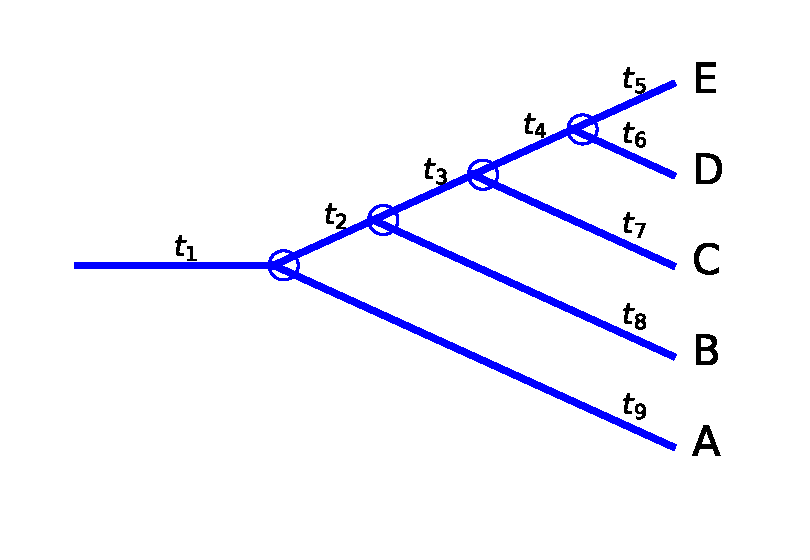
\includegraphics[width=\textwidth]{AncillaryFiles//figure1.eps}
\caption{A phylogenetic tree} \label{fig1}
\end{center} 
\end{figure}

There are a large number of other possibilities as well, even though the structure of the tree constrains some sorts of events. For example, an additional plausible sequence of migratory events would be for an initial migratory episode from C to A, followed by another from C to B, followed by yet another migration from C to D or E.

\begin{figure}
\begin{center} 
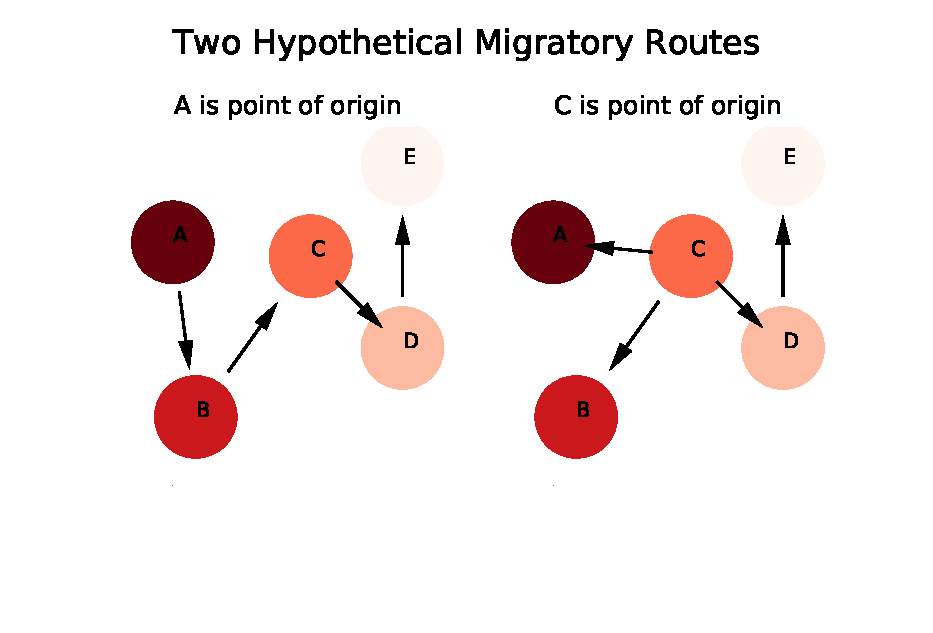
\includegraphics[width=\textwidth]{AncillaryFiles//figure2.eps} 
\caption{Potential migratory routes among a language stock consisting of five groups, following the Phylogenetic Tree in figure.} \label{fig2}
\end{center} 
\end{figure}

These two possible migratory routes are presented in figure \ref{fig2}. The AAH suggests that the second sequence is a less likely migratory history than the sequence. Why? For a variety of reasons - one might simply appeal to Occam's razor - the events on the left-hand side of figure \ref{fig2} require only one migratory chain, while the events on the right-hand side require three separate expansions: an initial migration from A to C, followed by another from A to B. A third migratory event is sufficient to take care of the last two groups: it begins from C continues to D, and then to E. We can now pose our question as follows: if we believe these migratory events to be rare, and we wish to conserve them in explaining historical migrations, what sort of model would accomplish this? But can one make this operational in a more formal setting? Can one characterize parsimony in a meaningful mathematical and probabilistic way? 

\section{A model}

\subsection{Tree Basics}

Along these lines, assume that we observe the entire phylogenetic tree, and that there are no unobserved migratory events. The tree is assumed to be a full, rooted, binary tree, meaning that there is a single origin node and branch, and all other nodes have a single parent. In a binary tree, all the interior nodes have two children, and all terminal nodes (leaves) have zero children. 

A binary tree with $n$ leaves has $n-1$ internal nodes. The tree in figure \ref{fig1} has five terminal nodes and four internal nodes. Importantly, this also applies to subtrees, which means that if a node has $k$ ancestors, then it is followed by $k-1$ nodes.

\subsection{Migratory Chains}
 
I build the model around what I call a  \textit{migratory chain}. Roughly speaking, a migratory chain is a directed path from the root of the tree to an end node, which, once traversed, divides the tree into subtrees. Positing that a particular culture or society is the point of origin of the tree amounts to positing some sequence of migratory chains through the phylogenetic tree. \begin{assumptions}{Migratory Chains}    
\begin{enumerate}
\item Migratory chains are unique in the sense that each is governed by its own parameters. 
\item  A migratory chain can begin with any location that is currently occupied but only one is active at any given location at any given time. 
\item The location where the chain originates generates a mass-migration at time $t$ according to an exponential distribution with parameter $\lambda$.
\item The location emitting the mass-migration also emits its propensity to migrate. Put another way, this propensity to migrate is carried off with the mass-migrating group to its new location. 
\end{enumerate}
\end{assumptions}
I will call a mass-migration history originating at location $i$ $\mathcal{H}_i$, and we will consider only mass-migration histories requiring the minimal number of mass-migrations needed to explain the current distribution of cultures. As a practical matter, this means that each history will have exactly $n-1$ migrations. Each location for our terminal nodes $i=1,2,3,\hdots I$ then will come along with a $\mathcal{H}_i$. We will refer to the number of migratory chains corresponding with $\mathcal{H}_i$ as $C_i$. 

The principal observation of forming a model in this fashion is now to use the ideas in definitions 1 to develop a probability corresponding with a history of migratory chains, and to relate this to some notion of distance between societies to prove an Age Area Theorem, which will come in the form of relationships between $\mathcal{H}$, $\mathcal{C}$, and $\mathcal{P}$, the probability that point $i$ is the point of origin for the societies in $I$. 

To preview the basic logic, I  develop a comparison of the two scenarios described in figure \ref{fig2} within the confines of the model. I begin by assuming that we do not know the exact times at which branching events occur, but instead only know the basic structure of the tree. But I will start as treating these points as known and then ``integrating them out,'' replacing the Exponential model with a Poisson model. 

The first scenario requires an initial migratory event to start after time $t_0$ from point $A$. At this point, according to the model assumptions, $A$ is dormant, and the migratory bug is passed to location $B$. After time $t_1$, $B$ sends the migratory bug to $C$, followed by $C$'s emission and subsequent dormancy, and then $D$'s. Finally, $E$ retains the bug, which travels no further. The result of this sequence of events is that over the entire time span of the tree, there have been exactly 4 migratory events associated with the one necessary migratory chain. In assumptions 1, this means that only one parameter is required to explain this particular migratory history. The probability of this sequence of events then follows a Poisson distribution with four occurrences over the whole time spanned by the tree $T$:
\begin{equation} \label{l1}
P_a = \frac{(\lambda\ T)^4
e^{-4T}}{4!}\end{equation} 
Which is labelled as $P_a$ because it is effectively the probability of this one migratory chain occurring.\footnote{Note that there is a slight abuse of notation here. One might argue that we should include the probability of migratory events in general occurring, or write the above as a conditional probability where we are really talking about $P(a|N_m=1)$.} The log-likelihood associated with the above is:
\begin{equation} \label{l2}
\ln P_a  = 4\ln(\lambda T) -4T-\ln(4!)
\end{equation} 
Differentiating \ref{l2} with respect to $\lambda$, and solving gives $\lambda^*=\frac{4}{T}$, and substituting this back into the objective function gives the likelihood as:
\begin{equation}  \label{l3}
P_a=\frac{4^4e^{-4}}{4!}
\end{equation}

There are a couple of points of interest about equation (\ref{l3}). First, since only one migratory chain is needed to explain the sequence of events, only one parameter is needed for the whole process. In this sense, this a parsimonious - it requires only one distribution and one parameter. 

Contrast this with the case in which $C$ is the initial location of the culture area. To maintain consistency with the linguistic or genetic analysis, we require 1) a migratory chain that starts at $C$ and goes to $A$, 2) a migratory chain that starts at $C$ and goes to $B$, and then 3) a migratory chain that starts at $C$ and proceeds to $D$ (or $E$) and then finally to $E$ (or D). According to the model, each of these chains requires its own Poisson/exponential distribution and parameter, which results in a likelihood of:
\begin{equation} \label{l4}
P_{c}=\frac{(\lambda_1t)^1e^{-\lambda_1t}}{1!}\frac{(\lambda_2(t-t_0))^1e^{-1}}{1!}
\frac{(\lambda_3(t-t_0-t_1))^2e^{-\lambda_3(t-t_0-t_1)}}{2!}
\end{equation} 
Maximizing $P_c$ in (\ref{l4}) with respect to $\lambda_1,\lambda_2$ and $\lambda_3$, and substituting the result back into the right-hand side of (\ref{l4}) gives:
\begin{equation} \label{l5}
P_{c}=\frac{1^1e^{-}}{1!}\frac{1^{1}e^{-1}}{1!}\frac{2^2e^{-2}}{2!}=
\frac{2^2e^{-4}}{2!}
\end{equation} 

According to equation (\ref{l5}), the relative likelihood that $A$ is the point of origin relative to $C$ depends upon $P_a /(P_a+P_c$), which, roughly put is a race between the functions $\frac{4^4}{4!}$ and $\frac{2^2}{2!}$. If for some reason we had restricted things to these two possibilities, the relative probability that $A$ was the point of origin would then be 84\%. 
A key feature of the previous analysis is the function 
\begin{equation*}
a(n)=\frac{n^n}{n!}
\end{equation*}
which is convex in $n$. This convexity, which owes to the structure of the Poisson distribution, implies that one is better off with explanations that require fewer parameters and that lump migratory events into longer chains. Hence, in a very precise sense parsimonious explanations are deemed more likely. Conversely, breaking up a migratory chain into two smaller chains eschews this convexity, and results in a less believable or less likely explanation. That is, for any  $k \in (1,n-1)$, it is true that:
\begin{equation*}
a(n) > a(n-k)a(k)
\end{equation*} 

There are a details that need to be fleshed out, but the above example illustrates the essentials of the model. The biggest detail that needs to be worked out is how the above theory that longer migratory chains are more parsimonious and therefore more likely relates to a measure of linguistic divergence. This task and others is taken up in the next section.

\begin{definition}{Divergence:}
Let $N^*$ denote the maximum number of migratory events that can be touched off from a location $i$, and let $C^*$ denote the minimum total number of chain migrations needed to explain all current locations if $i$ is the location of origin. Then, define Divergence of language $i$ :
\begin{equation*}
D_i=\frac{N^*}{C^*}
\end{equation*}
\end{definition}


\section{ Age-Area Theorem}

\begin{theorem}[Age-Area Theorem]
Suppose that the above model of chain migration as rare events holds described in Assumptions 1 holds, and define linguistic divergence as above in Definition 1. Then,  
\begin{equation*}
D_i \geq D_j \Longleftrightarrow p_i\geq p_k
\end{equation*}
and in particular
\begin{equation*}
i=\argmax\left[D_1,D_2,D_3,\hdots,D_n\right] \Longleftrightarrow i=\argmax\left[p_1,p_2,p_3,\hdots,p_n\right]
\end{equation*}
\end{theorem}
\begin{proof}

Observe first that the probability that $i$ is the point of origin is a product of the functions $a$, which are convex in the number of migrations covered by a migratory chain. Thus, if $C_i$ chains are required, the length of each are $N_i$, we may write:
\begin{equation*}
p_i=\prod_{i=1}^{C_i} a(N_i)
\end{equation*} 
The proof is virtually completed by the convexity of $a(N)$, as breaking any chain into two smaller chains is a losing proposition, 
\end{proof} 

\section{Micro foundations}

Pursuant to the theorem, one might ask: what sort of process might produce a model like this of migration? One can actually develop a model that creates random scarcity, which incites mass migration. The trick is developing a theory in such a way so that it preserves migrations. That is, one requires that migrations move forward probabilistically and stops. Here is one way of doing this. 

Imagine that there are a large, nonbinding set of viable locations in the migratory universe. At some an initial point, a new event arrives. This creates a system-wide increase in resources. 

At a particular point in the universe of places, imagine we imagine that income per capita depends upon a resource and also the current number of inhabitants. That is, flow per capita income at a particular location is
\begin{equation}
y_t=f(n_t,\theta_t)
\end{equation} 
Suppose that when income is above some subsistence level $s$ population increases proportionally. (This can be derived from a standard model). Normalize the subsistence level to unity. Then, in a given instant of time, current population creates additional population so long as their is additional income. That is, we have:
\begin{equation*}
n_{t+\Delta}=n_t\left(f(n_t,\epsilon_{t+\Delta}-\epsilon_{t})
-1)\Delta+n_t
\end{equation*}

Let's further suppose that $f(n_t,\epsilon_t,\epsilon_{t+\Delta})$ can be captured by a first-order Taylor expansion so we get:
\begin{equation*}
n_{t+\Delta}=n_t\left(\overline{f}+f_1n_t-s+f_2(\epsilon_{t+\Delta}-\epsilon_t)})
-1)\Delta+n_t
\end{equation*}

If we let $\Delta $ go to zero, and suppose that $\epsilon$ is governed by a standard brownian motion, we can write the above as a stochastic differential equation of the form:

\begin{equation*}
dn=n(\overline{f}+f_1n-s)+f_2^2n^2dz
\end{equation*}
We can reparameterize this by supposing that $\overline{f}=r$, $f_1=\frac{r}{K}$, and $f_2=\sigma$. The result is then a stochastic logistic population growth model:

\begin{equation}
dn=rn\left(1-\frac{n}{K}\right)+\sigma^2n^2dz
\end{equation} \label{sde}

The exact parameterization of the model is not necessary; what is important is that the mean-reverting nature of the SDE in equation (\ref{sde}) has a time-independent, stationary distribution, as \cite{rdgn99} note. This distribution is given by:
\begin{equation*}
W(n) = \Gamma\left[\frac{2a}{\sigma^2}-1\right]^{-1}\left(\frac{2b}{\sigma^2}\right)^{\frac{2a}{\sigma^2}-1}x^{\frac{2a}{\sigma^2}-2}\exp\left[\frac{2bx}{\sigma^2}\right]
\end{equation*}
Note to self. $\sigma$ has the same meaning, and $a=r$, while $b=r / K$. If we plug this in, the above gets quite simple. 

As \cite{rdgn99} and \cite{nrs99} show, the existence of a time-independent steady state density implies that the time to hitting a remote barrier is approximately exponential: that is:
\begin{equation*}
g(S,t|n) \sim \frac{1}{t_1(S,y)}\exp\left(-\frac{t}{t_1(S|y}\right) 
\end{equation*}

Armed with these facts, we can now create a version of the model that produces migratory chains that are approximately exponentially distribution. So, consider the following back story for the model.
\begin{enumerate}
\item The landscape is uniform in that all locations have the same initial carrying capacity $K_0$. 
\item A new migratory chains raises the carrying capacity across all locations to $K_1>$K_0$. 
\item There is a catch; if the population should ever reach the high boundary $S$, the carrying capacity immediately reverts to $K_0$. 
\end{enumerate}

The above sequence of events lead to a temporal population surplus. Suppose that a mass-migration requires a certain level of population $\overline{p}$ without which it will not succeed. The


\begin{figure}
\begin{center}
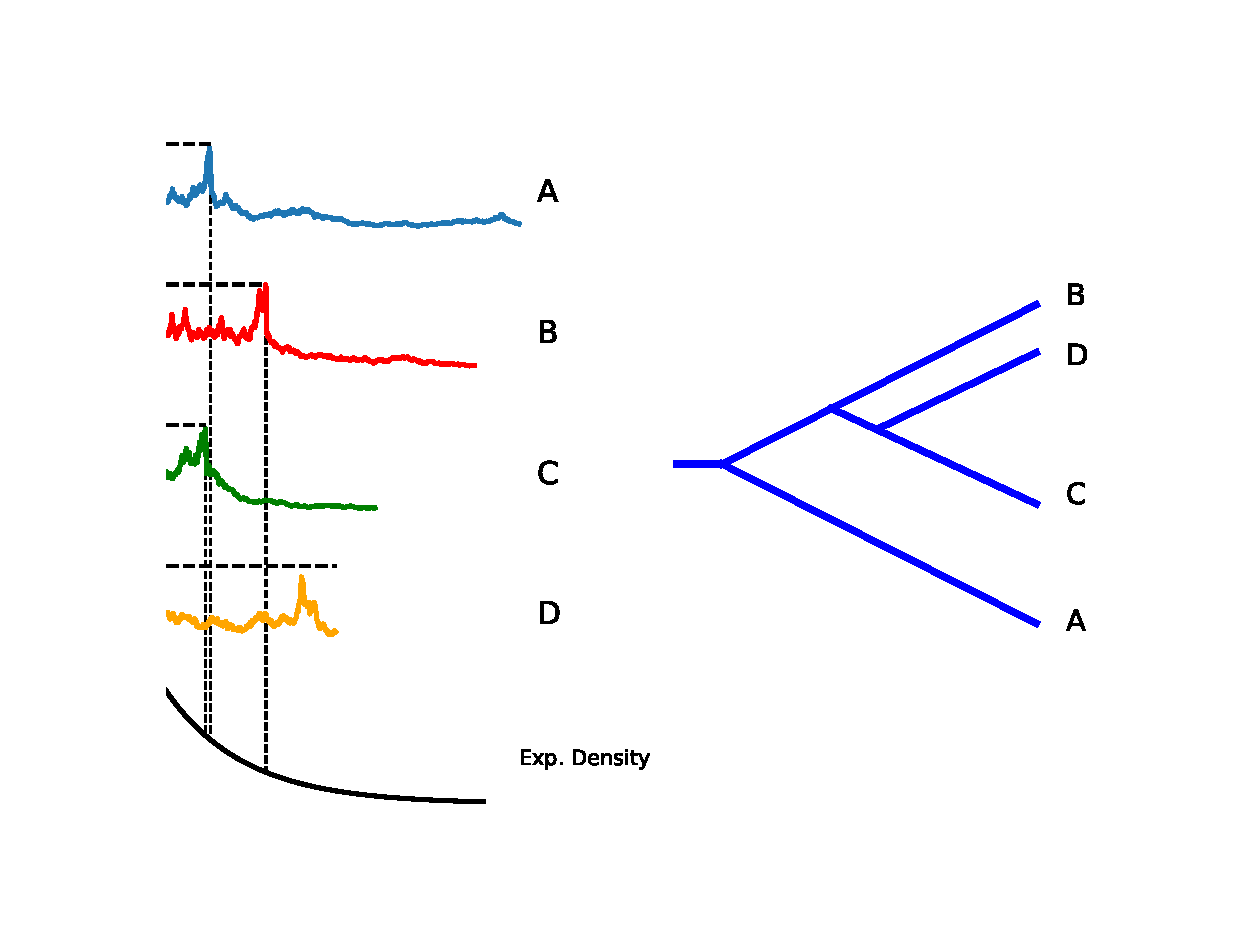
\includegraphics[width=\textwidth]{AncillaryFiles//figure3.eps}
\caption{An illustration of the formation of a phylogenetic tree. The left-hand side of the figure denotes times at which the barrier is hit, triggering mass migrations. Note that the length of the tree corresponds with the length of the path starting at $A$, which is also the same as the sums of the other branches.} \label{fig1}
\end{center} 
\end{figure}


s is often the case when dealing with estimation over trees, it behooves one to consider an algorithm that works backwards from the branches to the base. The algorithm presented here is essentially a pruning algorithm like Felsenstein's with a hint of dynamic programming. The dynamic programming aspect introduces a sort of continuation maximum likelihood into the tree.

The algorithm works as follows. At termination, the result is a concentrated log-likelihood of each location being the point of origin.  The following is an illustration showing how the algorithm works on the example given above.

\begin{enumerate}
\item[0.] Initialization: a ``active'' vector of zeros $A=[0,0,0,0,0]$, a vector of exponential parameters that start with zero, $E=[0,0,0,0,0]$, and a continuation likelihood $L=[-t_4,-t_5,-t_6,-t_7,-t_8]$
\item  Select an interior node and pick out its branches.
\item  Poo I\ can add stuff again! \end{enumerate}

\cite{gildner91}
\cite{dowd09}\cite{rdgn99}





\bibliographystyle{apalike}
\bibliography{bibfile}

\end{document} 
